% !TEX root = ../main.tex
\section{Introduction}
\label{sec:intro}

Agents built on large language models solve tasks in turns: the model reads the conversation so far, emits a tool call, and continues from the tool's observation~\citep{yao2023react}.
With a reasoning model, every turn first thinks through the situation, often for hundreds of tokens, before it emits its call.
A single customer-service task then takes minutes, and almost all of this time is the model's own generation, one turn after another.

Recent work removes the part of this time that is spent waiting for tools.
Speculative tool dispatch predicts the call while the model is still reasoning and executes it at once, so that the observation is ready when the model asks for it~\citep{nichols2025speculative,sui2026paste,bai2026spork}.
In its self-speculative form, the prediction comes from the target model itself and needs no training~\citep{bai2026spork}.
But this hides only the tool latency.
When a tool answers within seconds and a turn reasons for much longer, little is gained: with the \ToolLowFloor\,s tool latency of prior evaluations~\citep{bai2026spork}, speculative tool dispatch saves \DetSaveDispNone\% of the end-to-end time in our experiments.
The next turn still starts only when the current turn has finished.
A second line of work does start future steps early, but it takes them from a separate proposer, a cheaper agent or a trained drafter, that must guess what the target model will decide~\citep{hua2024isp,guan2025dsp,ye2026speculative,xu2026leap}.
Its gain depends on how often the proposer agrees with the target, and a trained proposer has to be fitted to each workload.

We start from the time that remains once the tool is off the critical path.
With speculative tool dispatch, a correct call is dispatched in \MotAnchorPct\% of the tool-calling turns, and its observation is ready after a median of \MotReadyPosPct\% of the turn's generation time.
The model then keeps reasoning until it writes the same call, a pattern that has also been reported by \citet{anon2026eta}.
We call this remaining time the \emph{slack} and find two properties of it (\cref{sec:motivation}).
First, the slack is long enough to cover much of the following turn. The median ratio of slack to next-turn duration is \MotSlackOverNext, and on average \MotNextCoveredPct\% of the next turn would fit into it.
Second, the input of the next turn is already determined.
The history keeps only the final output of a turn and not its reasoning, so the next input consists of the conversation so far, the call, and its observation.
Built from the dispatched call, it is identical to the real next input, token by token, in \MotInputSamePct\% of these turns.
During the slack, the agent thus waits for the model to confirm a call that has already been executed, while everything the next turn needs is at hand.

We present \method, which uses the slack to run the next turn (\cref{fig:overview}).
As soon as the observation of the dispatched call is ready, \method starts the next turn on the same target model, from the input that would follow if the current turn ended with exactly this call.
When the current turn finishes, \method keeps the early turn only if its input is identical to the real next input.
Otherwise it discards the early turn and runs the next turn as usual.
Three strategies make this safe.
\stratLaunch starts the next turn at the observation of the dispatched call, so that it builds on a real tool result and not on a predicted one.
\stratSandbox runs the tool calls of unconfirmed turns on copies of the environment, so that a discarded turn leaves no trace.
\stratCommit accepts the early turn only if its whole input matches token by token.
When decoding is deterministic, a committed turn is then exactly the turn that serial execution would have produced.
\method needs no training and no second model, because the early turn is the target model's own turn.

We evaluate \method on the airline and retail domains of \taubench with Qwen3-32B.
Under deterministic serving, it reduces the mean task time by \DetSaveOursDisp\% compared with speculative tool dispatch (\DetSpeedOursDisp$\times$) and by \DetSaveOursNone\% compared with the serial loop, and all configurations produce the same trajectory, token for token, on every task.
Under standard serving, the saving over speculative tool dispatch is \StdSaveOursDisp\%, with comparable gold-action match rates.
A cost model with a single measured parameter, the slowdown of two concurrent requests, predicts both savings from runs without \method (\CostDetPred\% and \CostStdPred\%).
It also states when the method pays off: the share of overlap time spent on committed successors must exceed the relative cost of the second request.
Longer tool latencies leave less slack for the successor. On the same ablation tasks, its incremental saving falls to \ToolHighIncrement\% at a \ToolHighFloor\,s tool floor.

Our contributions are as follows.
\begin{itemize}[leftmargin=*,itemsep=2pt,topsep=3pt]
\item We show that an agent with speculative tool dispatch spends about half of its end-to-end time (\MotSlackWallPct\%) in slack, that the slack can hold most of the next turn, and that a correctly dispatched call and its observation determine the input of the next turn in \MotInputSamePct\% of the cases.
\item We propose \method, a training-free method that runs the next turn of the target model inside the slack, with sandboxed tool execution and an exact-input commit rule that leaves the trajectory unchanged under deterministic decoding.
\item We show that \method reduces the task time by \DetSaveOursDisp\% over speculative tool dispatch with identical trajectories, and we give a cost model that explains its savings under two serving modes.
\end{itemize}

% Draft rendering from scripts/fig_overview.py; to be replaced by the hand-drawn vector figure.
\begin{figure*}[t]
\centering
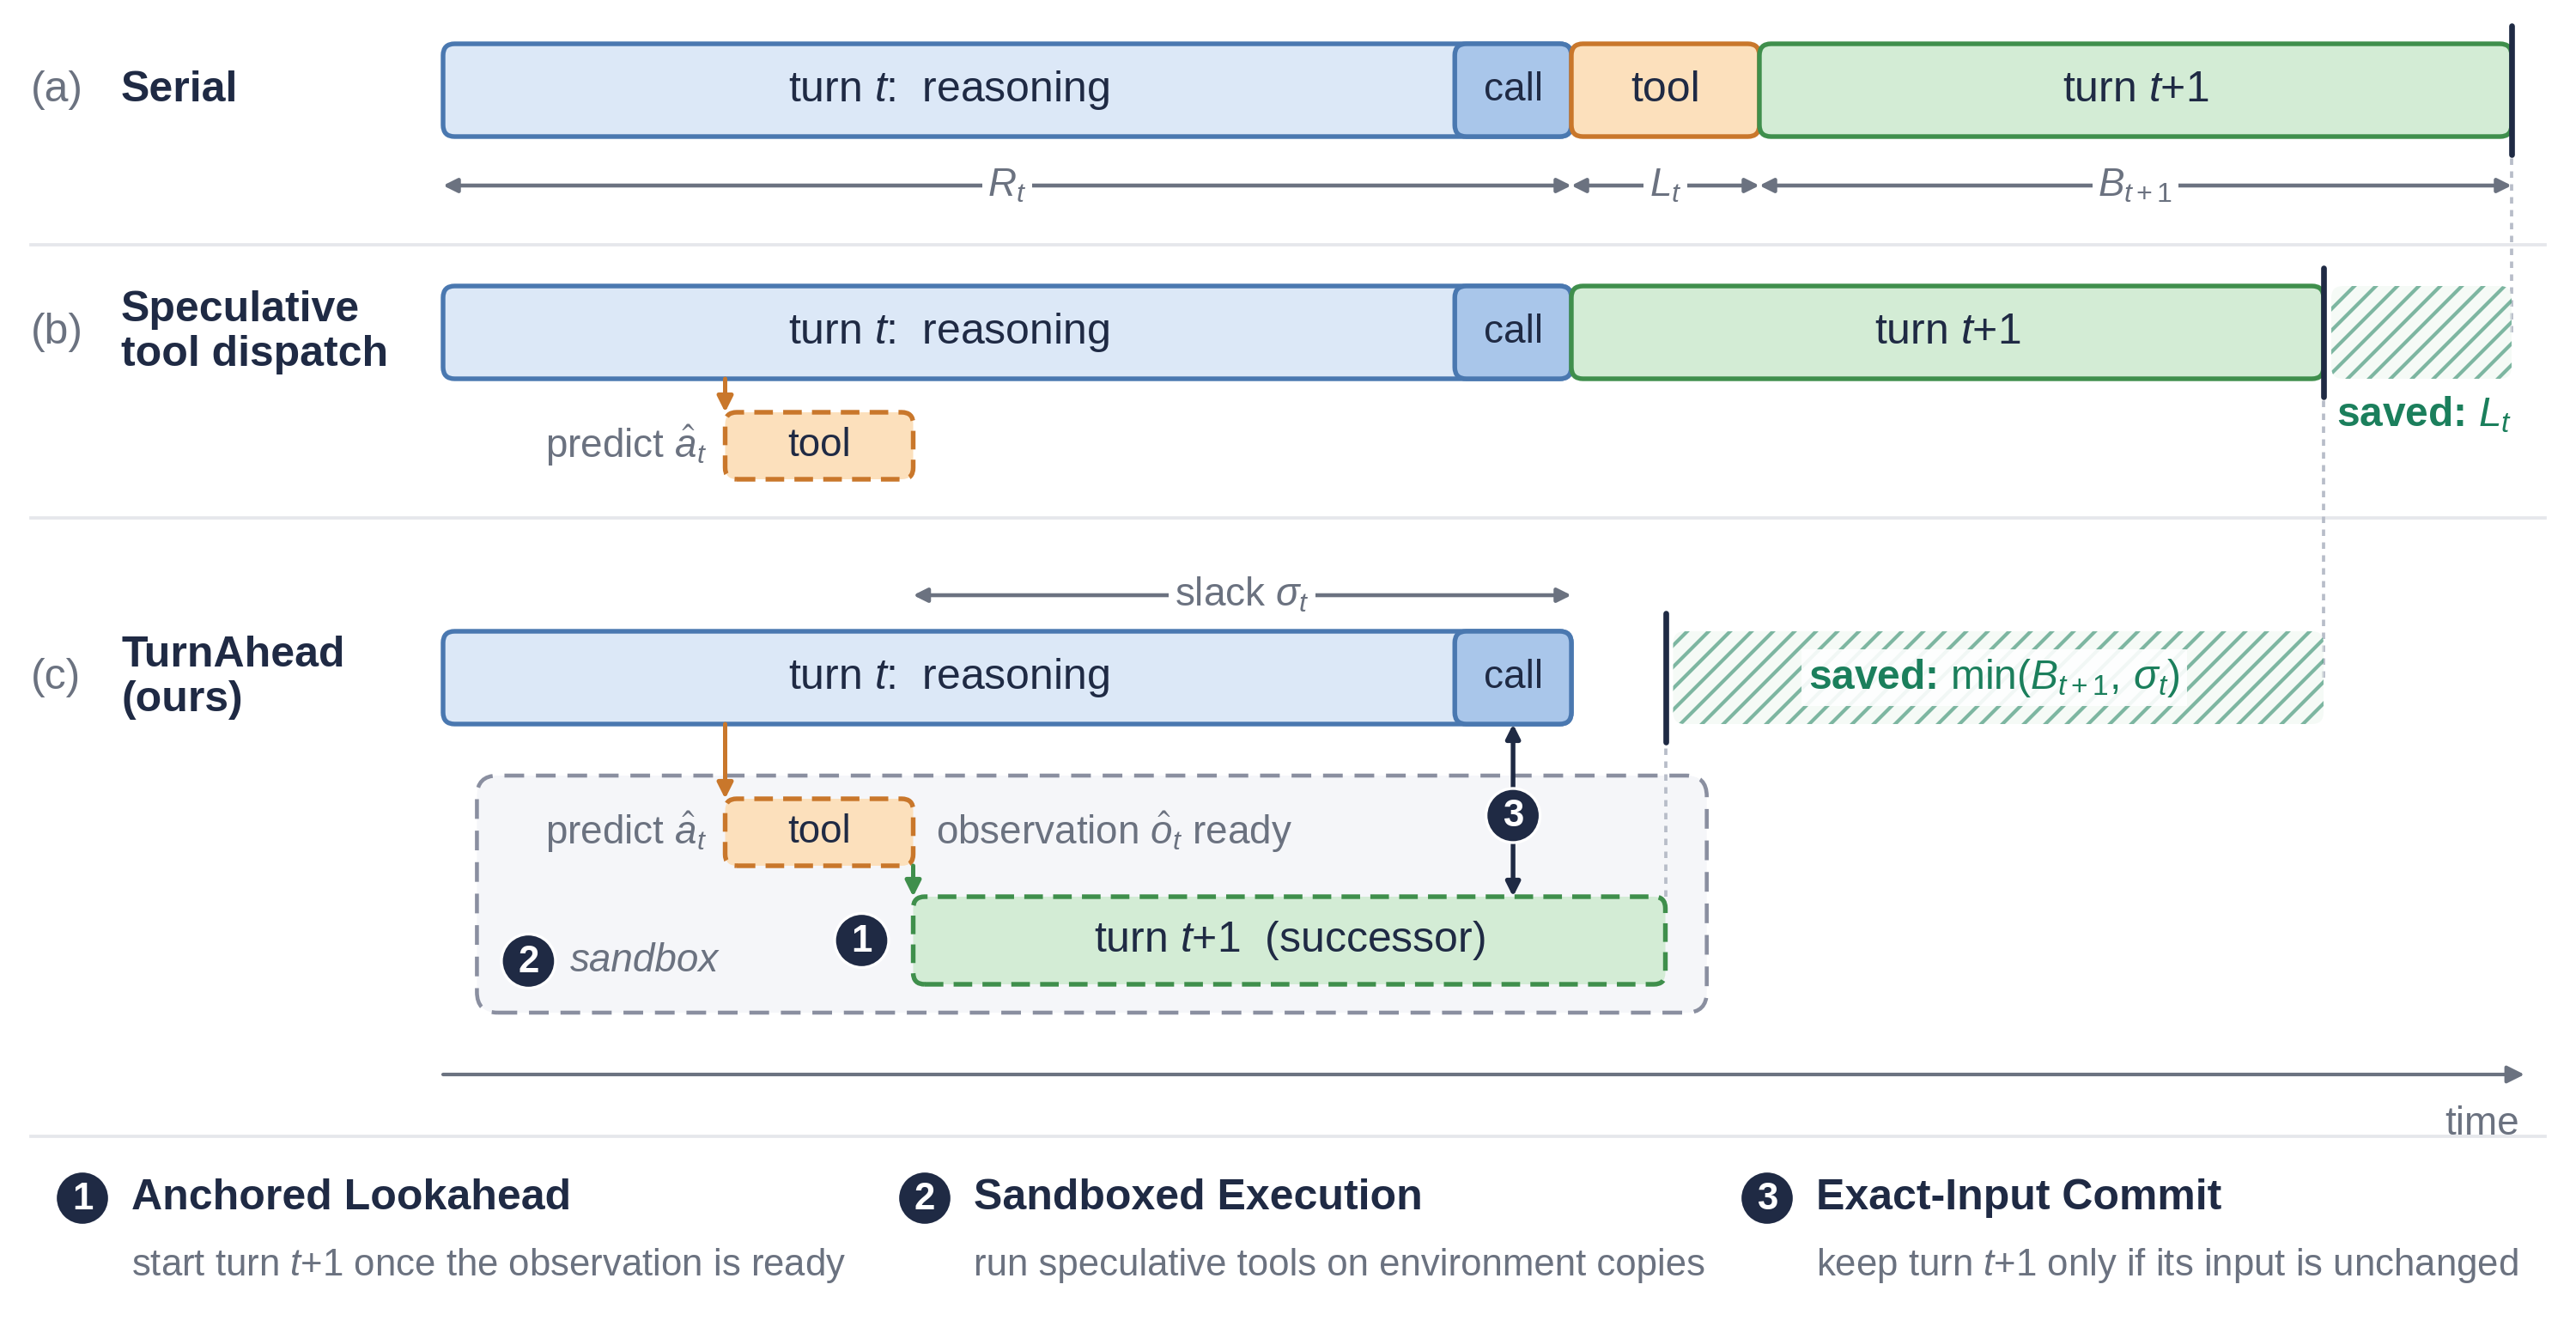
\includegraphics[width=\textwidth]{figures/fig1_overview.png}
\caption{One window of two turns. (a) Serial execution. (b) Speculative tool dispatch predicts the call during reasoning and hides the tool latency $L_t$. (c) \method also starts turn $t{+}1$ once the observation is ready, runs it in a sandbox, and keeps it only if its input is unchanged when turn $t$ ends. Durations are illustrative.}
\label{fig:overview}
\end{figure*}
